\documentclass[12pt, a4paper]{article}

\usepackage[T1]{fontenc}
\usepackage[utf8]{inputenc}
\usepackage{amsmath, amssymb, amsfonts, amsthm}
\usepackage{bbm}
\usepackage{graphicx}
\usepackage{verbatim}
\usepackage{caption}
\usepackage{subcaption}
\usepackage{subfig}
\usepackage{float}
\usepackage{algorithm}
\usepackage{algpseudocode}

\theoremstyle{definition} \newtheorem*{definition}{Teorem}

\newcommand{\vb}{\mathbf}
\newcommand{\lla}{\left \langle}
\newcommand{\rra}{\right \rangle}

\renewcommand{\contentsname}{Innhald}

\renewcommand{\abstractname}{Samandrag}

\renewcommand{\figurename}{Figur}

\renewcommand{\tablename}{Tabell}

\makeatletter
\newcommand{\newalgname}[1]{
    \renewcommand{\ALG@name}{#1}
}
\newalgname{Algoritme}

\begin{document}

\begin{titlepage}
    \begin{center}
        \vspace*{1cm}
        
        \textbf{\huge Molekylær Dynamikk}

        \vspace{0.5cm}
        \textbf{Oblig 3}

        \vspace{1cm}
        av

        \vspace{1cm}
        \textbf{Øyvind Sigmundson Schøyen} \\
        Kandidatnummer: 30 \\

        \vspace{2.0cm}

        Avsluttande prosjekt i FYS3150 \\

        \vspace{1.5cm}

        \includegraphics[width=0.4\textwidth]{\string~/Downloads/UiO_Segl_300dpi.png}

        \vspace{1.0cm}

        FYS3150 Computational Physics\\
        Det matematisk-naturvitskaplege fakultet\\
        Universitetet i Oslo\\

        \vfill

        Desember 2014

    \end{center}
\end{titlepage}

\begin{abstract}
    I dette prosjektet har me tatt for oss modellering av Argon på atomært nivå. Me har vore interesserte i å lage eit program som skal lage ein atomstruktur etter eige ynskje.
    I tillegg har me ville sjå på korleis eit slikt system utvikler seg over tid og måle statistiske eigenskapar ved det. For å modellere eit så realistisk resultat
    som mogleg har me nytta cellelister for å auke hastigheita på programmet. For krafta har me nytta Lennard Jones potensialet og som integrator
    har me brukt Velocity Verlet-algoritma. Programma våre er objektorientert \verb!C++!-kode med eit \verb!Python! rammeverk som skal enklast mogleg køyre programmet vårt for forskjellige 
    parametrar og plotte verdiar. Me nyttar VMD for å visualisere atoma i rommet. All kjeldekode ligg på github.\\ \\
    \texttt{https://github.com/Schoyen/molecular-dynamics-fys3150}
\end{abstract}

\newpage
    \tableofcontents
\newpage

\section*{Introduksjon}
    \addcontentsline{toc}{section}{Introduksjon}

    I dette prosjektet har me modellert eit fysisk system samt bruke objektorientert programmering for å halde ein ryddig, oversiktlig, samt effektiv kode. 
    I byrjinga er me gjeve ein kode som lagar 100 argon atom og gjer dei ein tilfeldig retning og hastighet. Gjeve lang nok tid vil atoma drive vekk. Me vil difor nytte
    ``periodiske randbetingelsar'' for å halde atoma i nærleiken. Grunna hastigheitar gjevne frå Maxwell-Bolzmann distribusjon vil systemet ha ein ikkje-null
    rørslemengde som me vil fjerne. Me vil deretter lage ein krystallstruktur kor me startar simuleringa av atoma. I eit slik lukka system vil total energien vere bevart, 
    men grunna numerisk avrunding er det ikkje alltid dette held mål. Ein stabil alogritme som me vil nytte er ``Velocity Verlet'' som er ein symplektisk integrator. % Forklar dette.
    Me vil no byrje å måle statistiske eigenskapar som energi og temperatur. For å kunne køyre koden for store system vil me derimot utvikle ein kjappar algoritme når 
    me rekner ut krafta mellom atompara. Dette løyser me med cellelister. Til slutt, i fyrste del av prosjektet, legg me til ein termostat som let oss kontrollere 
    temperaturen i systemet. \\ \\
    % Fyll in for del 2 av prosjektet.
    God lesning!



\newpage


\section*{Fysikken bak molekylær dynamikken}
    \addcontentsline{toc}{section}{Fysikken bak molekylær dynamikken}
    I denne delen av rapporten vil me sjå på dei forskjellige eigenskapane me måler i MD-koda vår. Eventuelle måleresultat vil bli vist i resultat-seksjonen.

    \subsection*{Oppsett}
        \addcontentsline{toc}{subsection}{Oppsett}
        Systemet med atom me set opp krev nokre tilpassningar for å gje eit realistisk resultat. 

        \subsubsection*{Face-Centered Cubic Lattice}
            \addcontentsline{toc}{subsubsection}{Face-Centered Cubic Lattice}
            Det fyrste me vil gjere å plassera atom i ein krystallstruktur. For Argon
            vil me då nytte ``face-centered cubic lattice'' (FCC). Me plasserer fire og fire atom i ei einingscelle. Posisjonane til kvart atom vil vere gjeve ved
            \begin{align*}
                &\vb{r}_1 = 0\vb{i} + 0\vb{j} + 0\vb{k}, \\
                &\vb{r}_2 = \frac{b}{2}\vb{i} + \frac{b}{2}\vb{j} + 0\vb{k}, \\
                &\vb{r}_3 = 0\vb{i} + \frac{b}{2}\vb{j} + \frac{b}{2}\vb{k}, \\
                &\vb{r}_4 = \frac{b}{2}\vb{i} + 0\vb{j} + \frac{b}{2}\vb{k}.
            \end{align*}
            Her vil $b$ vere ein konstant, me skal seinare sjå på korleis trykket er avhengig av denne. \\ % Hugs å legg dette ved i resultatet.

        \subsubsection*{Maxwell-Boltzmann og fartsmoment}
            \addcontentsline{toc}{subsubsection}{Maxwell-Boltzmann og fartsmoment}
            Etter at atoma vert plasserte i einingscellene vil me gje dei ein liten starthastighet kor me nyttar Maxwell-Boltzmann distribusjon. Då vil
            \begin{align*}
                \vb{v} \propto \sqrt{T}.
            \end{align*}
            Hastigheita til atoma vil bli fordelte tilfeldig i rommet. Resultatet er at systemet har eit ikkje-null fartsmoment. Før me byrjar å rekne ut nye posisjonar vil
            me fjerne dette fartsmomentet. Me vil då finne den totale hastigheita til systemet og trekke denne frå kvart atom.
            \begin{align*}
                &\vb{V} = \frac{1}{M}\sum_i^N m_i\vb{v}_{i}^{\text{før}}, \\
                &\vb{v}_{i}^{\text{etter}} = \vb{v}_{i}^{\text{før}} - \vb{V}, \qquad \ i \in [1, N],
            \end{align*}
            kor $\vb{V}$ er den total hastigheita til systemet, $N$ er antal atom, $M$ er den totale massa til alle atoma summert opp. Dette bidrar til at systemet vårt
            ikkje har ein total hastigheit, men heller står i ro. \\



        \subsubsection*{Lennard Jones}
            \addcontentsline{toc}{subsubsection}{Lennard Jones}
            For å få ein fysisk effekt på systemet må me byrje å rekne ut krafta mellom atoma. Me nyttar Lennard Jones potensialet for å finne krafta mellom atompara.
            Lennard Jones har den eigenskapen at potensialet tek med den fråstøytande og den tiltrekkande krafta mellom para. Potensialet er gjeve ved
            \begin{align*}
                U(r_{ij}) = 4\epsilon\left[ \left( \frac{\sigma}{r_{ij}} \right)^{12} - \left( \frac{\sigma}{r_{ij}} \right)^{6} \right],
            \end{align*}
            kor $r_{ij}$ er avstanden frå atom $i$ og $j$, $\sigma$ og $\epsilon$ er konstantar som bestemmer kva distanse potensialet er null og kor djup potensialbrønnen skal vere.
            Me finn krafta ved å ta den negative gradienten til potensialet. Då får me
            \begin{align*}
                \vb{F}(\vb{r}_{ij}) &= -\nabla U(r_{ij}) = -\frac{\partial U(r_{ij})}{\partial r_{ij}} \\
                &= -4\epsilon\left[ 12\left( \frac{\sigma^{12}}{r_{ij}^{14}} \right) - 6\left( \frac{\sigma^6}{r_{ij}^8} \right) \right]\vb{r_{ij}}.
            \end{align*}
            Grunna dei høge potensane kan me sjå at denne krafta vil kjapt gå mot null. Denne eigenskapen gjer at me kan effektivisere koda vår ved berre å rekne ut krafta 
            mellom atom kor avstanden mellom dei er innenfor ein radius $r_{\text{cut}}$.
            Eit plott over $U/\epsilon$ mot $r_{ij}/\sigma$ vil gje oss ein indikator kva tid krafta vil vere null.
            \begin{figure}[H]
                \centering
                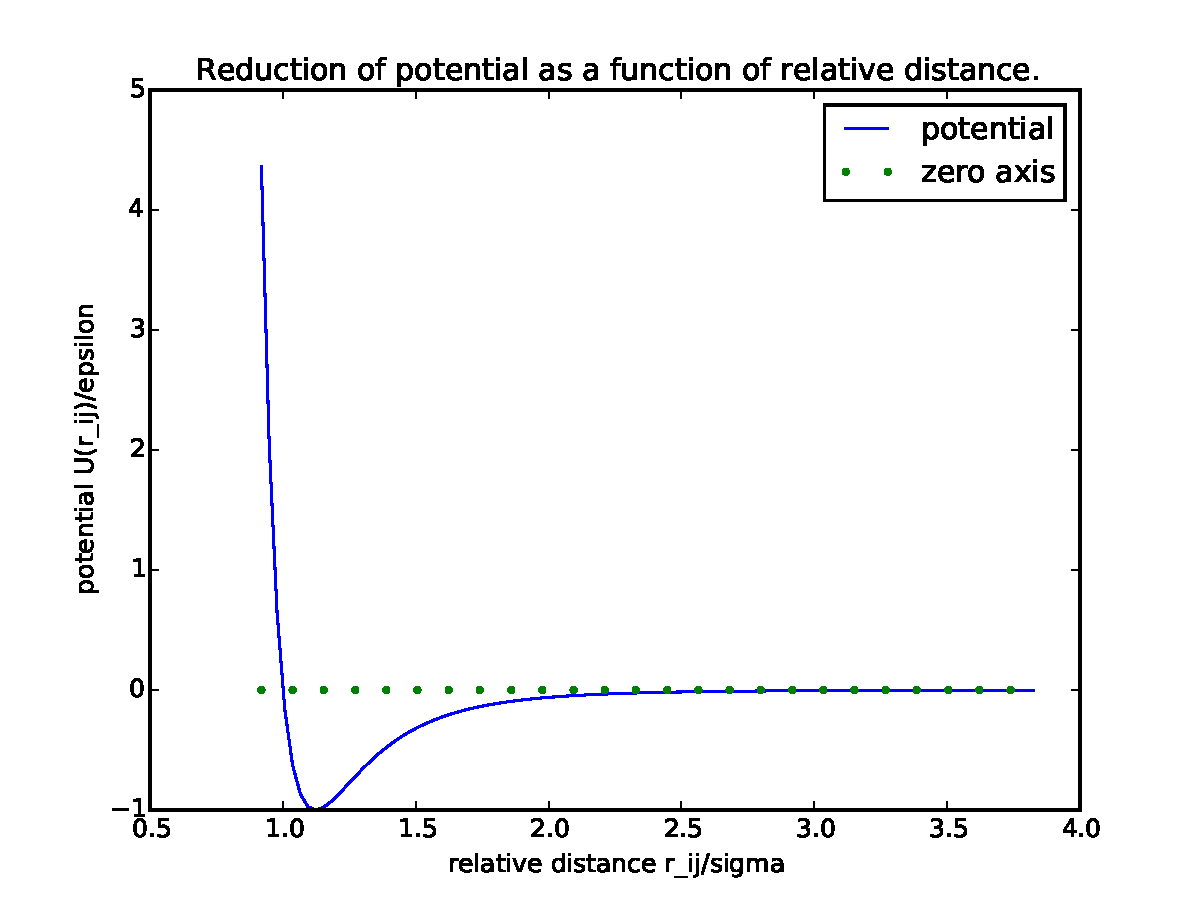
\includegraphics[width=400px]{potentialPlot.pdf}
                \caption{I plottet kan me lett sjå kor dei tiltrekkjande og kor dei fråstøytande kreftene har sine styrker. Då krafta er gjeve som den negative gradienten til
                        potensialet vil me kunne sjå at i det atoma kjem veldig nære einannan vil det virke ei kraftig fråstøyting ($r_{ij}^{12}$-delen) medan det for større avstand
                        vil virke ei svakare, men med større rekkevidde, tiltrekkande kraft ($r_{ij}^6$-delen).}
            \end{figure}
            Frå figuren les me av 
            \begin{align*}
                \frac{r_{\text{cut}}}{\sigma} \approx 2.5 \qquad \Rightarrow \qquad r_{\text{cut}} \approx 2.5\sigma.
            \end{align*}
            Utanfor denne radiusen vil me ikkje rekne krafta mellom atompara.


    \newpage

    \subsection*{Statisiske målingar}
        \addcontentsline{toc}{subsection}{Statistiske målingar}
        Hensikten med koda vår er for å måle eigenskapar i eit system med atomar.

        \subsubsection*{Energi}
            \addcontentsline{toc}{subsubsection}{Energi}
            Det enklaste å måle vil vere energien i systemet. Me har allereie implementert eit uttrykk for den potensielle energien med Lennard Jones. Då finner me
            den kinetiske energien ved formelen
            \begin{align*}
                E_{k} = \sum_{i}^N\frac{1}{2}m_iv_{i}^2,
            \end{align*}
            kor $N$ er antal atomar i systemet. Total energien vil då vere gjeve ved
            \begin{align*}
                E = E_{k} + U.
            \end{align*}
            For eit system av atom med dei randbetingelsane me har satt forventer me energibevaring. Grunna numerisk avrunding vil det alltid oppstå små fluktuasjonar,
            men desse forventer knapt skal vere synlege. \\

            Då me ikkje reknar krafta mellom atompar utanfor $r_{\text{cut}}$ må me endre litt på Lennard Jones potensialet slik at me har energibevaring. 
            Potensialet vil nå bli skalert etter likninga
            \begin{align*}
                U_{\text{skalert}}(r_{ij}) = 
                \begin{cases}
                    U(r_{ij}) - U(r_{\text{cut}}), & r \leq r_{\text{cut}} \\
                    0, & r > r_{\text{cut}}.
                \end{cases}
            \end{align*}

        \subsubsection*{Temperatur}
            \addcontentsline{toc}{subsubsection}{Temperatur}
            Temperaturen speler ei stor rolle i systemet vårt. Me er interesserte i å finne ut kva tid strukturen smelter og kor tid ho held seg stabil. Me finn ho 
            ved ekvipartisjonsteoremet som seier
            \begin{align*}
                &\left \langle E_{k} \right \rangle = \frac{3}{2} Nk_{B}T \qquad \Rightarrow \qquad T = \frac{2}{3}\frac{E_{k}}{Nk_{B}},
            \end{align*}
            kor $T$ då angjer den momentane temperaturen då me ikkje tek gjennomsnittet av $E_{k}$. Temperaturen vil fluktuere då den kinetiske energien vil endre seg for
            kvart tidssteg. Etterkvart vil me nå eit stabilt likevektspunkt kor temperaturen held seg nokonlunde jamnt.


        \subsubsection*{Nummertettleik}
            \addcontentsline{toc}{subsubsection}{nummertettleik}
            Me vil måle tettleiken til systemet til å vere antal atomar delt på volumet til heile systemet. Dette vil vere ein konstant, men me vil sjå på korleis denne vil 
            endre seg som ein funksjon av konstanten $b$ som me nyttar ved konstruksjon av einingscellene til systemet. Storleiken på systemet vil vere gjeve ved
            \begin{align*}
                V = S_xS_yS_z,
            \end{align*}
            kor $V$ er volumet til systemet og $S_x$, $S_y$ og $S_z$ er lengda til kvar av sidene til systemet. Då finner me tettleiken ved
            \begin{align*}
                \rho_N = \frac{N}{V},
            \end{align*}
            kor $N$ er antal atomar i systemet. Me vil og finne eit uttrykk for nummertettleiken som ein funksjon av konstanten $b$ som avgjer astand mellom atoma i 
            einingscellene. Då får me at
            \begin{align*}
                \rho_N = \frac{N}{V} = \frac{N}{S_xS_yS_z}.
            \end{align*}
            Storleiken på systemet i dei forskjellige retningane er gjeve ved likningane
            \begin{align*}
                S_x &= bN_{FCCX}, \\
                S_y &= bN_{FCCY}, \\
                S_z &= bN_{FCCZ},
            \end{align*}
            kor $N_{FCC}$ avgjer kor mange einingsceller i kvar dimensjon me vil ha. Då ser me at 
            \begin{align*}
                \rho_N = \frac{N}{V} = \frac{4N_{FCCX}N_{FCCY}N_{FCCZ}}{b^3N_{FCCX}N_{FCCY}N_{FCCZ}},
            \end{align*}
            då fylgjer det at
            \begin{align*}
                \rho_N = \frac{4}{b^3}.
            \end{align*}


        \subsubsection*{Trykk}
            \addcontentsline{toc}{subsubsection}{Trykk}
            Trykket til systemet er gjeve ved formelen 
            \begin{align*}
                P = \rho_Nk_BT + \frac{1}{3V}\left \langle \sum_{i = 1}^N \vb{F}_{i}\cdot\vb{r}_{i} \right \rangle,
            \end{align*}
            kor $\rho_N$ er tettleiken, $k_B$ er Boltzmann konstanten, $T$ er temperaturen, $V$ er volumet til systemet og $\vb{F}_i$ og $\vb{r}_i$ er henholdsvis krafta
            og posisjonen til atom $i$. Då me nyttar Newtons tredje lov (N3L) i kraftutrekninga vår vil me kunne forenkle dette uttrykket og istaden rekne ho ut inne i kraftløkka.
            Me kan for parvis interaksjon skrive krafta om til å vere
            \begin{align*}
                \sum_i^N \vb{F}_i\cdot\vb{r}_i &= \sum_i\sum_{j\neq i}\vb{r}_i\cdot \vb{F}_{ij} \\
                &= \frac{1}{2}\sum_i\sum_{j\neq i }\left( \vb{r}_i\cdot\vb{F}_{ij} + \vb{r}_j\cdot\vb{F}_{ji} \right) \\
                &= \frac{1}{2}\sum_i\sum_{j\neq i}(\vb{r}_i\cdot\vb{F}_{ij} - \vb{r}_j\cdot\vb{F}_{ij}) \\
                &= \frac{1}{2}\sum_i\sum_{j\neq i}( (\vb{r}_i - \vb{r}_j)\cdot\vb{F}_{ij}) \\
                &= \frac{1}{2}\sum_i\sum_{j\neq i} \vb{r}_{ij}\cdot\vb{F}_{ij} \\
                &= \sum_i\sum_{j > i}\vb{r}_{ij}\cdot\vb{F}_{ij},
            \end{align*}
            kor $\vb{F}_{ij}$ og $\vb{r}_{ij}$ er krafta og avstanden mellom atom $i$ og $j$. Me set dette inn i uttrykket for trykk.
            \begin{align*}
                P = \rho_Nk_BT + \frac{1}{3V}\left \langle \sum_{i > j} \vb{F}_{ij}\cdot\vb{r}_{ij} \right \rangle.
            \end{align*}


        \subsubsection*{Varmekapasitet}
            \addcontentsline{toc}{subsubsection}{Varmekapasitet}
            Varmekapasiteten er eit mål på kor mykje varme eit materiale kan lagre medan det skjer ei temperaturendring. Me kan rekne ut varmekapasiteten ved å nytte variansen 
            i kinetisk energi. Me har då eit forhold som seier
            \begin{align*}
                \lla E_k^2 \rra - \lla E_k \rra^2 = \frac{3Nk_B^2T^2}{2}\left( 1 - \frac{3Nk_B}{2C_V} \right),
            \end{align*}
            kor $k_B$ er Boltzmann konstanten, $T$ er temperatur og $C_V$ er varmekapasiteten. Me vil omforme denne likninga slik at me får varmekapasiteten for seg sjølv på 
            venstre sida. Me får då
            \begin{align*}
                &\lla E_k^2 \rra - \lla E_k \rra^2 = \frac{3Nk_B^2T^2}{2} - \frac{9N^2k_B^3T^2}{4C_V}, \\
                &\Rightarrow \qquad -4C_V\left( \lla E_k^2 \rra - \lla E_k \rra^2 -\frac{3Nk_B^2T^2}{2}\right) = 9N^2k_B^3T^2, \\
                &\Rightarrow \qquad C_V = -\frac{9N^2k_B^3T^2}{4\left( \lla E_k^2 \rra - \lla E_k \rra^2 -\frac{3Nk_B^2T^2}{2}\right)}.
            \end{align*}
            Me vil måle denne verdien i eininga $\frac{\text{J}}{\text{Kmol}}$ for å samanlikne med eksperimentelle verdiar. Boltzmann konstanten er gjeve ved
            \begin{align*}
                k_B \sim \frac{\text{m}^2\text{kg}}{\text{s}^2\text{K}} \sim \frac{\text{J}}{\text{K}}.
            \end{align*}
            Då ser me at vermakapasiteten vil vere gjeve ved
            \begin{align*}
                C_V \sim \frac{\left( \frac{\text{J}}{\text{K}} \right)^3\text{K}^2}{\text{J}^2 - \text{J}^2 - \left(\frac{\text{J}}{K})\right)^2\text{K}^2} 
                \sim \frac{\text{J}}{\text{K}}.
            \end{align*}
            For å finne mol må me difor gonge antal atomar med $\textbf{Avogrados konstant}$.
            Denne er gjeve ved
            \begin{align*}
                k_A = 6.02214129\times10^{23}\text{ mol}^{-1}.
            \end{align*}


    \subsection*{Berendsen termostat}
        \addcontentsline{toc}{subsection}{Berendsen termostat}
        Siden temperaturen fluktuerer vil me gjerne ha moglegheit til å styre ho. Me vil implementere ein $\textbf{Berendsen termostat}$. Ho er gjeve ved 
        \begin{align*}
            \gamma = \sqrt{1 + \frac{\Delta t}{\tau}\left( \frac{T_{\text{bath}}}{T} - 1 \right)}.
        \end{align*}
        Skaleringsfaktoren $\gamma$ vil me gonge med hastigheita $\vb{v}$ til atoma i systemet. Her er $\tau$ ein parameter som avgjer kor kjapt temperaturen skal endrast.
        $T_{\text{bath}}$ er den ønska temperaturen medan $T$ er den noverande temperaturen. Me kan då sjå at $\gamma = 1$ for $T = T_{\text{bath}}$. Desverre er ikkje dette
        ein veldig realistisk termostat då temperaturen endrer seg mykje fortare enn det ville skjedd i virkelegheita. Dette gjer blant anna at me ikkje vil måle fysiske eigenskapar
        så lenge termostaten er på. Me vil difor nytte ho for å nå ei ynskja temperatur for så å la systemet få stabilisere seg litt før me byrjar å måle verdiar.


\newpage


\section*{Algoritmar}
    \addcontentsline{toc}{section}{Algoritmar}

    \subsection*{Simulering av eit uendeleg stort system}
        \addcontentsline{toc}{subsection}{Simulering av eit uendeleg stort system}
        Då me ikkje kan simulere eit uendeleg stort system vil me nytte nokre metodar kor me slepper å sjå at atoma våre forsvinn ut i ingenting.

        \subsubsection*{Periodiske randbetingelsar}
            \addcontentsline{toc}{subsubsection}{Periodiske randbetingelsar}
            Viss eit atom har ein 
            posisjon som ligg utanfor storleiken på systemet vårt vil me flytte atomet slik at det kjem inn frå den andre sida av systemet. For eit stort system kan dette 
            vere ei god tilnærming då det heile tida forsvinn atom ut frå eit lite område, men samstundes kjem det inn nye atom slik at tettheten er jamn. Dette vil og vere med
            på å gje oss bevaring av total energi då det ikkje går noko tap til vegger og liknande. Periodiske randbetingelsar vil vere gjeve ved formelen
            \begin{align*}
                \vb{r}_i = x_i\vb{i} + y_i\vb{j} + z_i\vb{k}, \qquad i \in [1, N],
            \end{align*}
            kor $N$ er antal atom i systemet. Då vil kvar komponent i $\vb{r}_i$ vere gjeve ved
            \begin{align*}
                x = 
                \begin{cases}
                    x + S_x, & x < 0 \\
                    x, & x \in [0, S_x) \\
                    x - S_x, & x \geq S_x
                \end{cases},
            \end{align*}
            kor $S_x$ er storleiken på systemet i $x$-retning og $x$ er noverande posisjon for atomet. Me gjentek dette for dei to andre retningane og.



        \subsubsection*{Avstand frå endepunkta}
            \addcontentsline{toc}{subsubsection}{Avstand frå endepunkta}
            Frå analogien ved bruk av periodiske randbetingelsar må me ta hensyn til at avstand mellom atompar ikkje nødvendigvis stemmer. Argumentet vårt er at 
            atoma som ligg heilt i kanten av systemet har ``tvillingar'' som kjem inn frå andre sida på nøyaktig same tid og med dei same parametrane som seg sjølve.
            Når me då rekner avstand mellom atoma vil me sjekke om eigentleg ligg mykje nærare viss det eine atomet vert flytta over på den andre sida av systemet.
            Me kjem til å nytte ``Minimum Image Criterion'' for å sjekke om dette er oppfylt. Me definerer
            \begin{align*}
                \Delta \vb{R} = \vb{r}_i - \vb{r}_j, \qquad i \neq j, \qquad i, j \in [1, N],
            \end{align*}
            som gjer oss avstanden mellom atoma slik det framstår i simuleringa. For å simulere eit uendeleg system vil me difor sjekke om denne oppfyller krava
            \begin{align*}
                \Delta \vb{R} = \Delta X\vb{i} + \Delta Y\vb{j} + \Delta Z\vb{k},
            \end{align*}
            kor me har skrive $\Delta \vb{R}$ på komponentform. Då får me
            \begin{align*}
                \Delta X = 
                \begin{cases}
                    \Delta X - S_x, & \Delta X > \frac{S_x}{2} \\
                    \Delta X, & \Delta X \in \left( -\frac{S_x}{2}, \frac{S_x}{2} \right] \\
                    \Delta X + S_x, & \Delta X \leq -\frac{S_x}{2}
                \end{cases}
            \end{align*}




    \subsection*{Velocity Verlet}
        \addcontentsline{toc}{subsection}{Velocity Verlet}
        Idet systemet vårt er satt opp med ein starthastighet for kvart atom vil me tidsintegrere oss fram i tid for å sjå korleis det utvikler seg. Då systemet vårt er pakka
        inn med periodiske randbetingelser og biletekriterie vil me nytte ein algoritme som bevarer energien. Velocity Verlet er ein $\textbf{symplektisk integrator}$ som 
        bevarer total energien (Hamiltonian er bevart, men denne tilsvarer ofte total energien i eit system). Velocity Verlet er i tillegg ein enkel og kompakt algoritme med
        eit feilledd som går som $\mathcal{O}(\Delta t^2)$. Integrasjonen består av tre ledd
        \begin{align*}
            \vb{v}(t + \Delta t/2) &= \vb{v}(t) + \frac{\vb{F}(t)}{m}\frac{\Delta t}{2}, \\
            \vb{r}(t + \Delta t) &= \vb{r}(t) + \vb{v}(t + \Delta t/2)\Delta t, \\
            \vb{v}(t + \Delta t) &= \vb{v}(t + \Delta t/2) + \frac{\vb{F}(t + \Delta t)}{m}\frac{\Delta t}{2},
        \end{align*}
        kor me må rekne ut krafta ein gong for fyrste ledd før me byrjar å integrere oss fram i tid.

    \subsection*{Cellelister}
        \addcontentsline{toc}{subsection}{Cellelister}
        Det som er kostbart ved Velocity Verlet er utrekninga av kraft to gonger per ledd. Viss me rekner ut krafta mellom kvart atom vil me ha ei algoritme som går som
        $\mathcal{O}(N^2)$, kor $N$ er antal atom. Ved å sette opp cellelister vil me dele opp systemet vårt i mindre celler kor kvar side av cellene har lengde 
        $r_{\text{cut}}$ runda av til næraste heiltal. Ved å gjere dette slipper me å leite gjennom alle atoma i systemet vårt og rekne ut krafta mellom dei. Me vil 
        heller rekne ut krafta mellom atoma i ei celle og alle nabocellene til denne cella. Viss me då i tillegg sjekker om atoma i nabocellene ligg utanfor
        $r_{\text{cut}}$ vil me redusere køyretida til $\mathcal{O}(N)$.

        \begin{algorithm}[H]
            \caption{Rekn ut krafta ved hjelp av cellelister}
            \label{Cellelister}
            \begin{algorithmic}[1]
                \For {$i \in N_x$}
                    \For {$j \in N_y$}
                        \For {$k \in N_z$}
                            \State $Cell_{1} = CellIndex(i, j, k)$
                            \For {$cx \in \left[ i - 1, i + 1 \right]$}
                                \For {$cy \in \left[ j - 1, j + 1 \right]$}
                                    \For {$cz \in \left[ k - 1, k + 1 \right]$}
                                        \State $applyPeriodic(cx, cy, cz)$
                                        \State $Cell_{2} = CellIndex(cx, cy, cz)$
                                        \For {$m \in Cell_1.getAtoms()$}
                                            \For {$n \in Cell_2.getAtoms()$}
                                                \State Rekn ut krafta
                                            \EndFor
                                        \EndFor
                                    \EndFor
                                \EndFor
                            \EndFor
                        \EndFor
                    \EndFor
                \EndFor
            \end{algorithmic}
        \end{algorithm}
        Her er $N_x$, $N_y$ og $N_z$ antal celler i henholdsvis $x$-, $y$- og $z$-retning. $cx$, $cy$ og $cz$ viser til koordinatane til nabocellene. Metoden $applyPeriodic()$ 
        sjekker om cellene i endepunkta har naboar på andre sida av systemet. \\
        For kvart tidssteg må me legge atom i dei riktige cellene. Me lagrar cellene på indeksar gjeve ved formelen
        \begin{align*}
            index = iN_yN_z + jN_z + k,
        \end{align*}
        kor $i$, $j$ og $k$ er indeksane me sender inn. Då kan me finne kva celle eit atom høyrer til i ved å nytte formelen
        \begin{align*}
            index_x = \left \lfloor \frac{x_{\text{Atom}}}{S_{x}} N_{x}\right \rfloor,
        \end{align*}
        og tilsvarande for $y$- og $z$-retning. Då vil $index$-formelen over returnere cella som inneheld det gjeldane atomet.

\newpage
\section*{Struktur}
    \addcontentsline{toc}{section}{Struktur}
    I dette prosjektet har me nytta objektorientering for å halde styr på simuleringa vår. Simuleringane vert køyrde i \verb!C++!. Me har bygd eit rammeverk med 
    \verb!Python! som tek seg av køyringa i \verb!C++! for å gje eit betre overblikk. Litt diverse \verb!bash!-script rydder og strukturer utskriftar.

    \subsection*{Objektar i C++}
        \addcontentsline{toc}{subsection}{Objektar i C++}
        Under fylgjer ein kort oversikt over objekt me nyttar og formålet deira.

        \subsubsection*{Atom}
            \addcontentsline{toc}{subsubsection}{Atom}
            Filene $\texttt{atom.h}$ og $\texttt{atom.cpp}$ utgjer ein liten klasse kor me lagrar masse, posisjon, hastighet og krafta til eit atom. I tillegg 
            gjer me kvart atom ein indeks som gjer det mogleg for oss å nytte Newtons tredje lov kor me kun vil rekne ut krafta mellom para viss atom-objektet me
            har valgt har ein større indeks enn det andre atom-objektet me har valgt.

        \subsubsection*{Berendsen}
            \addcontentsline{toc}{subsubsection}{Berendsen}
            Programma $\texttt{berendsen.h}$ og $\texttt{berendsen.cpp}$ implementerer Berendsen termostaten beskrevet i seksjonen om fysikken bak molekylær dynamikken.
            Ho vert nytta av integratoren til å skalere hastigheita viss me vil ha kontroll over temperaturen.

        \subsubsection*{Cell}
            \addcontentsline{toc}{subsubsection}{Cell}
            Programma $\texttt{cell.h}$ og $\texttt{cell.cpp}$ vert nytta til å ta vare på atoma som ei einskild celle inneheld. Formålet med klassa er fyrst og fremst
            å kunne indeksere cellene slik at me kun treng å rekne ut krafta mellom ei og ei celle ein gong. Me slepp då å sjekke for kvart atom to for-løkker djupare.

        \subsubsection*{Cell List}
            \addcontentsline{toc}{subsubsection}{Cell List}
            Programma $\texttt{celllist.h}$ og $\texttt{celllist.cpp}$ inneheld ein vektor med Cell-objektar. Ho vil i tillegg lagre antal celler i $x$-, $y$- og $z$-retning.
            Klassa tek seg og av sorteringa av atom og legg dei inn i riktige celler.

        \subsubsection*{IO}
            \addcontentsline{toc}{subsubsection}{IO}
            Programma $\texttt{io.h}$ og $\texttt{io.cpp}$ tek seg av utskrift til fil i \verb!.xyz!-formatet. Dette formatet vert lese av VMD for visualisering av atoma.

        \subsubsection*{Statistics Sampler}
            \addcontentsline{toc}{subsubsection}{Statistics Sampler}
            Programma $\texttt{statisticssampler.h}$ og $\texttt{statisticssampler.cpp}$ inneheld metodar som lagrar og skriv ut dei fysiske eigenskapane me vil måle til fil.

        \subsubsection*{System}
            \addcontentsline{toc}{subsubsection}{System}
            Programma $\texttt{system.h}$ og $\texttt{system.cpp}$ er sjølve fundamentet blant objekta. Klassa handterer oppsett, køyring og lagrar atom. Ho handterer 
            sjølve gjennomføringa slik at eit main-program kun treng å køyre nokre få enkle metodar.

        \subsubsection*{Unit Converter}
            \addcontentsline{toc}{subsubsection}{Unit Converter}
            Programma $\texttt{unitconverter.h}$ og $\texttt{unitconverter.cpp}$ skalerer einingane på dei fysiske verdiane slik at me arbeider me meir handterlege tal.
            Dette gjer og moglegheita for store numeriske avrundingsfeil mykje mindre.

        \subsubsection*{Integrator}
            \addcontentsline{toc}{subsubsection}{Integrator}
            Programma $\texttt{integrator.h}$ og $\texttt{integrator.cpp}$ utgjer ein superklasse som tillater oss å nytte forskjellige numeriske integrasjonsalgoritmar.

        \subsubsection*{Velocity Verlet}
            \addcontentsline{toc}{subsubsection}{Velocity Verlet}
            Programma $\texttt{velocityverlet.h}$ og $\texttt{velocityverlet.cpp}$ er ein numerisk integrasjonsalgoritme som står forklart i algoritme seksjonen.

        \subsubsection*{Random}
            \addcontentsline{toc}{subsubsection}{Random}
            Programma $\texttt{random.h}$ og $\texttt{random.cpp}$ utgjer ein random-generator som me nyttar når me set starthastigheita til kvart atom med 
            Maxwell-Boltzmann distribusjon.

        \subsubsection*{Vec3}
            \addcontentsline{toc}{subsubsection}{Vec3}
            Programma $\texttt{vec3.h}$ og $\texttt{vec3.cpp}$ er ein lett vektorklasse som implementerer vektoroperasjoner for tre-dimensjonale vektorar. Styrken til klassa 
            er at me berre lagrar tre double-verdiar. Ho vil difor vere kjapp under runtime.

        \subsubsection*{Potential}
            \addcontentsline{toc}{subsubsection}{Potential}
            Programma $\texttt{potential.h}$ og $\texttt{potential.cpp}$ er ein superklasse, som på same måte som $\texttt{integrator.h}$ tillater bruk av forskjellige
            potensial. Klassa lagrar og den potensielle energien og summen av krafta og avstanden mellom atoma som me treng for å rekne ut trykket.

        \subsubsection*{Lennard Jones}
            \addcontentsline{toc}{subsubsection}{Lennard Jones}
            Programma $\texttt{lennardjones.h}$ og $\texttt{lennardjones.cpp}$ implementerer Lennard Jones potensialet og uttrykket for krafta. Her ligg og implementasjonen 
            av cellelister.


    \subsection*{Python-rammeverk}
        \addcontentsline{toc}{subsection}{Python-rammeverk}
        Grunna storleiken på programmet og dei forskjellige simuleringane me vil gjere er det enklare å køyre main-metoden frå \verb!Python!. Rammeverket består av ein klasse
        som køyrer kommandolinje-argument. Ho tek seg av køyring av Makefile og plottar og skriv ut til fil.
\newpage


\section*{Resultat}
    \addcontentsline{toc}{section}{Resultat}
    I resultata våre vil me sjå på både fysikken og køyretid på dei to forskjellige metodane me nyttar for å rekne ut krafta.

    \subsection*{Køyretid}
        \addcontentsline{toc}{subsection}{Køyretid}
        På køyretida har me ei slags forventning over kva som vil skje. Eg valgte å køyre programmet for eit aukande antal atom kor me gjer nyttar 1000 tidsskritt. Resultatet ligg
        i tabellen under.

        \begin{table}[H]
            \centering
            \begin{tabular}{|l|l|l|}
                \hline
                Antal atomar & Kraft mellom kvart atom & Cellelister \\
                \hline
                864 & 11\text{s} & 11 \text{s}\\
                2048 & 42 \text{s}& 24 \text{s}\\
                2916 & 77 \text{s}& 31 \text{s}\\
                4000 & 136 \text{s}& 39 \text{s}\\
                5324 & 228 \text{s}& 58 \text{s}\\
                6912 & 365 \text{s}& 69 \text{s}\\
                8788 & 576 \text{s}& 85 \text{s}\\
                10976 & 881 \text{s}& 114 \text{s}\\
                13500 & 1283 \text{s}& 133 \text{s}\\
                16384 & 1860 \text{s}& 173 \text{s}\\
                19652 & 2642 \text{s}& 198 \text{s}\\
                23328 & 3772 \text{s}& 241 \text{s}\\
                27436 & 5147 \text{s}& 279 \text{s}\\
                32000 & 6749 \text{s}& 316 \text{s}\\
                \hline
            \end{tabular}
            \caption{I tabellen står køyretida programmet treng for køyre antal atomar som står på venstre side. Antalet atom er bestemt ut frå likninga
                     $N = 4L^3$, kor $L$ er antal FCC gitter. Køyretida er oppgjeven i sekund. Me kan tydeleg sjå korleis cellelister held ei lineær stigning i
                     køyretid til skjelnad frå å rekne ut krafta mellom alle atoma.}
        \end{table}

        Eit plott over desse verdiane fylgjer under.
        \begin{figure}[H]
            \centering
            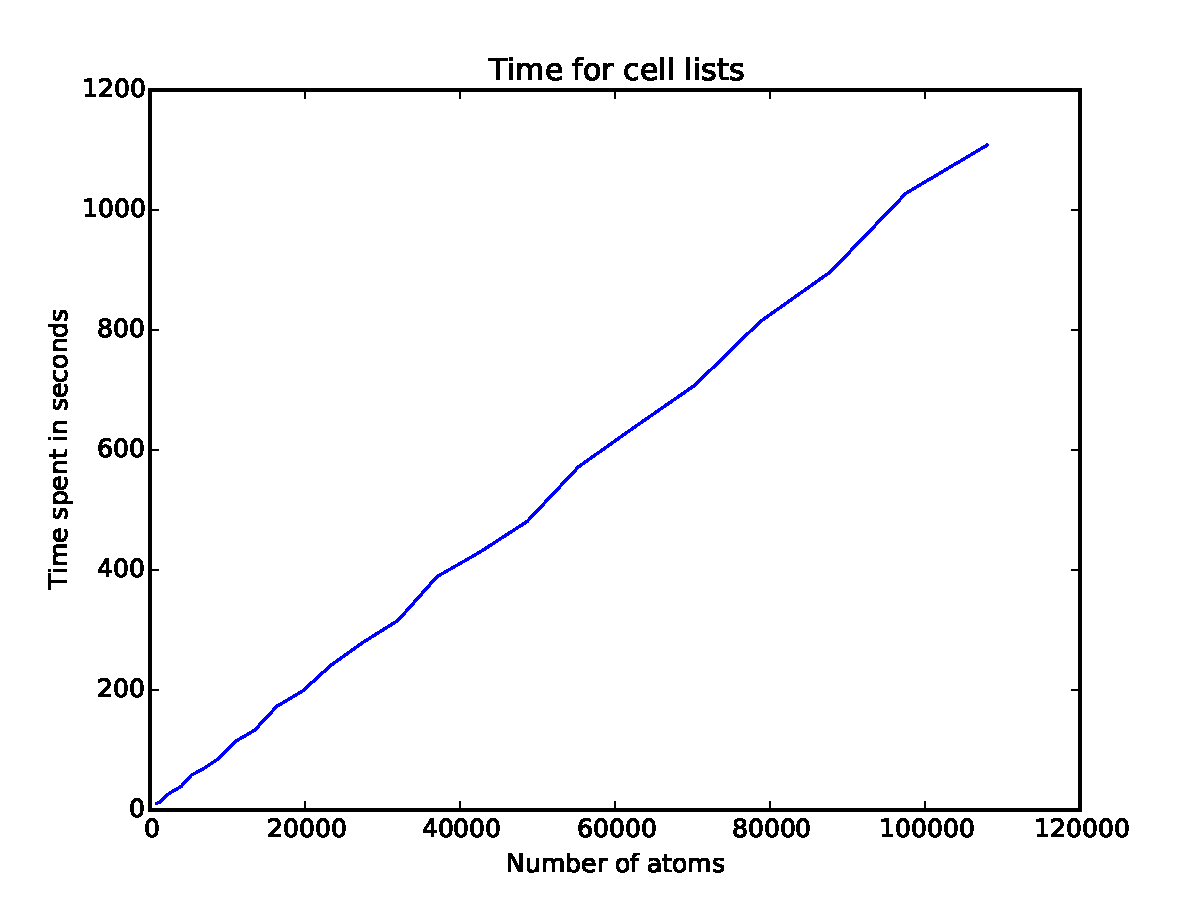
\includegraphics[width=400px]{cellListsTime.pdf}
            \caption{Her kan me sjå korleis cellelisten stig lineært med antal atom. Dette gjeld for dei betingelsane me har satt for $r_{cut}$.}
        \end{figure}

        \begin{figure}[H]
            \centering
            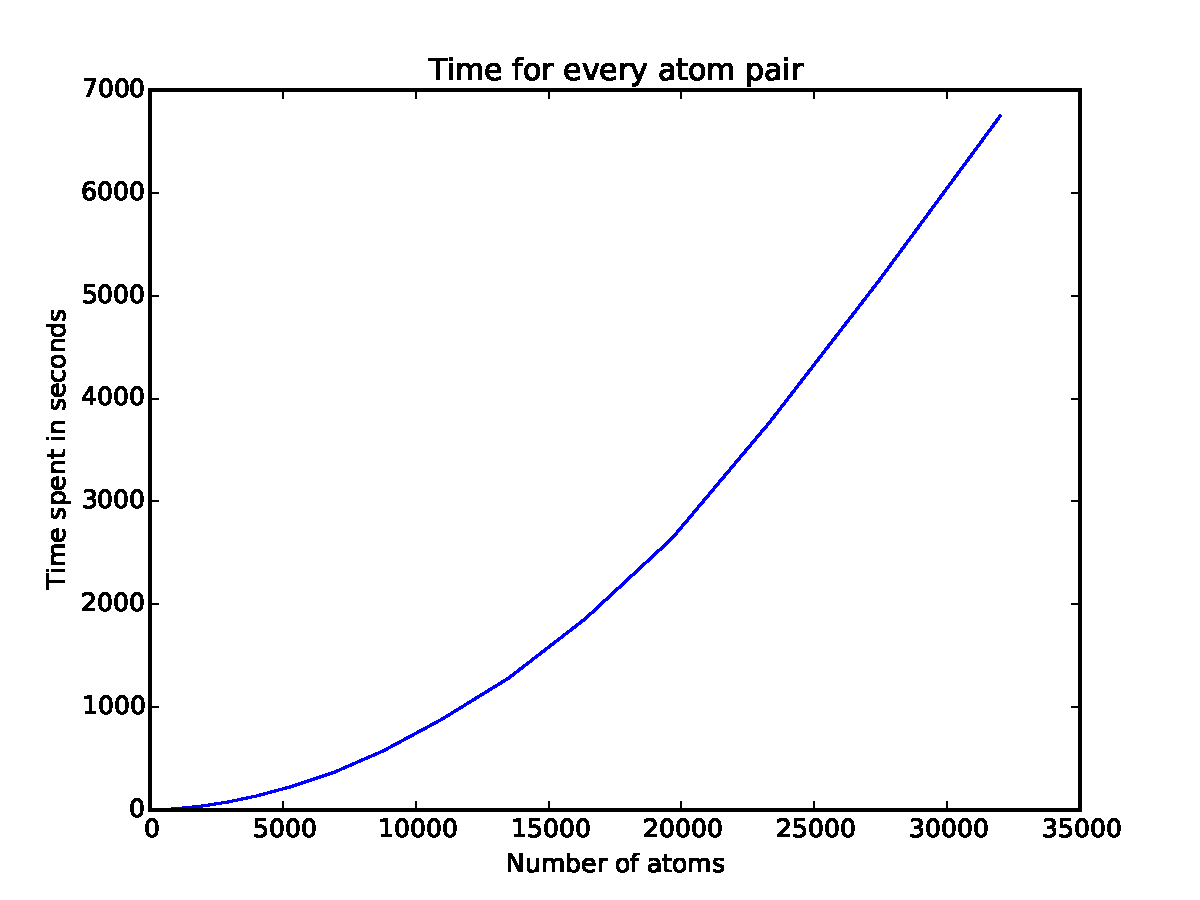
\includegraphics[width=400px]{oldForceTime.pdf}
            \caption{Me kan sjå at tida det tek å rekne ut krafta veldig fort vert stor.}
        \end{figure}
        Eg køyrde desse verdiane over 10 timar (HOLY SHIT) og har difor resultat frå høgare verdiar av cellelister. Diverre vert tida det tok å køyre programmet for den treige kraftmetoden
        for stor. Eit interessant mål vil vere å sjå kiloatom per tidsskritt. Me ser med andre ord på kor mange tusen atom metoda klarer å rekne ut for per tidsskritt. Under 
        fylgjer grafane for dei to metodane.

        \begin{figure}[H]
            \centering
            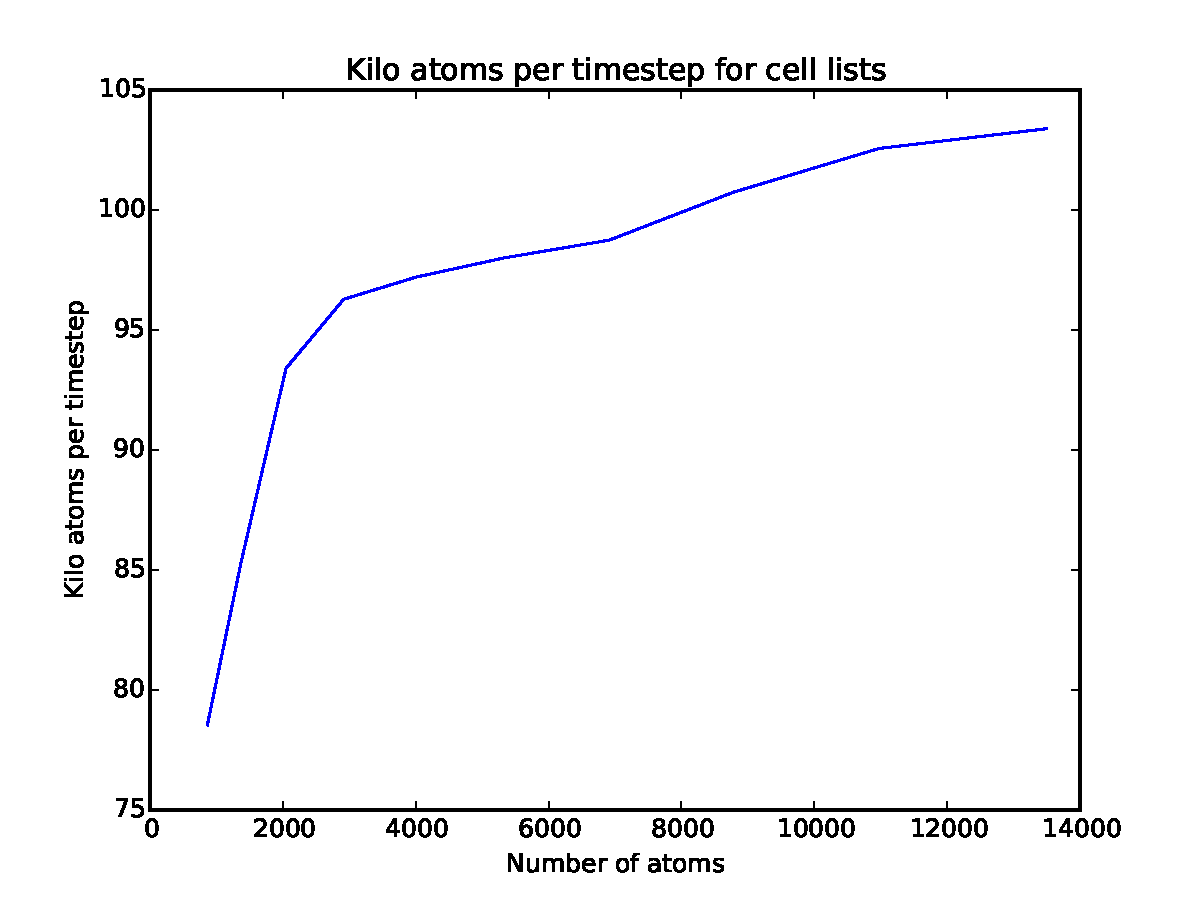
\includegraphics[width=400px]{cellLists.pdf}
            \caption{For cellelister kan me sjå at me i byrjinga får eit brått hopp opp. Dette skjer då metoda fyrst vert effektiv når me får ein viss storleik på cellelistene
                     i forhold til antal atom. Ho vil difor etterkvart stabilisere seg rimelig jamnt. Me får fluktuasjonar som kan skyljast ujamnt antal atom i kvar celle.}
        \end{figure}
        \begin{figure}[H]
            \centering
            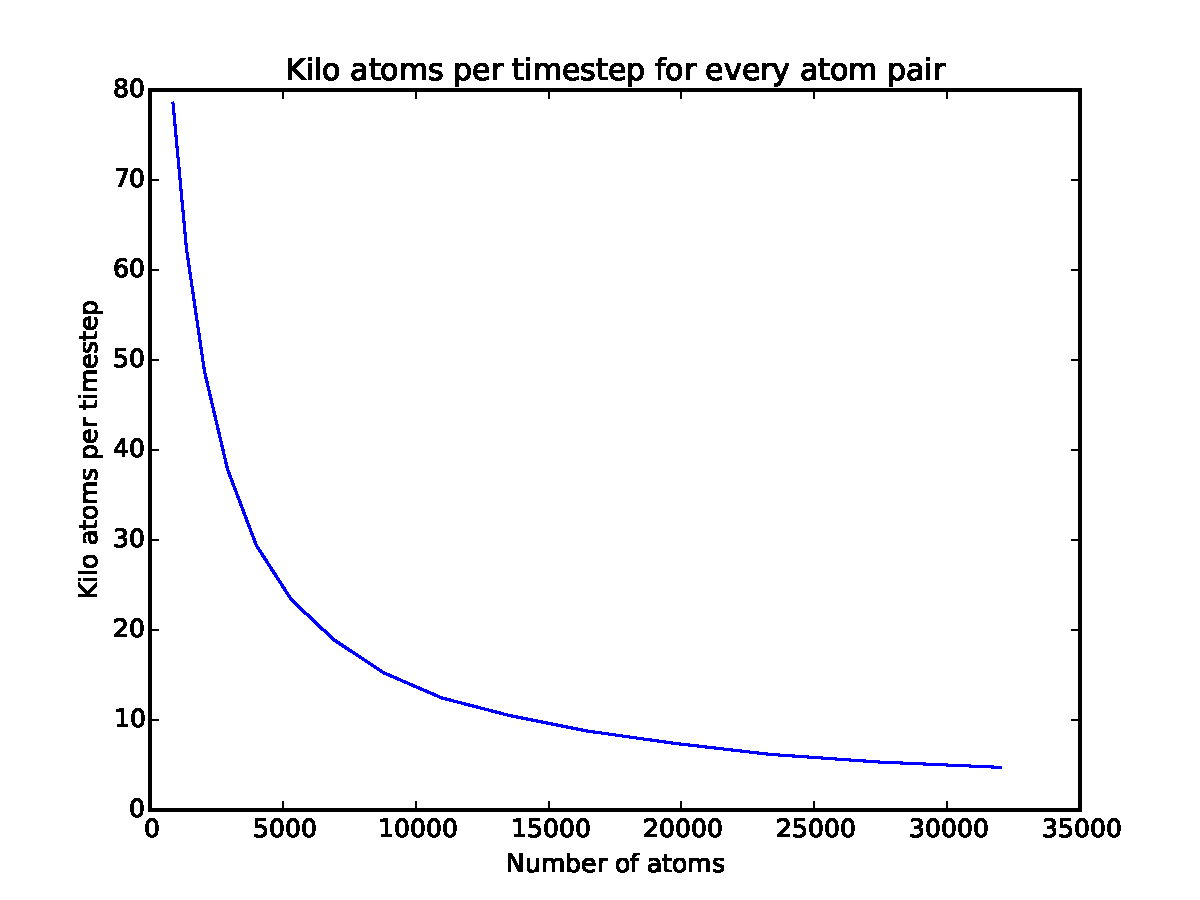
\includegraphics[width=400px]{oldForce.pdf}
            \caption{Ved å rekne krafta mellom kvart atom kan me sjå at metoda kjapt vil bli treig. Etterkvart klarer ho ikkje å rekne ut krafta mellom mange nok atom. Når me auker
                     antal atom vil ho slite med å rekne ut krafta mellom mange nok atom til at me vil klare å bli ferdige med utrekningane.}
        \end{figure}


    \subsection*{Fysikk}
        \addcontentsline{toc}{subsection}{Fysikk}

        \subsubsection*{Initial system}
            \addcontentsline{toc}{subsubsection}{Initial system}
            For å gje oss indikator av kva som skjer i simuleringa vår vil me køyre ein enkel, men lang, simulering kor me måler og analyserer dataene me får ut.
            Me set opp eit system på 4000 atomar og med ein starttemperatur på 300 K. Me simulerer for 20000 tidssteg.
            Då kan me sjå på korleis temperatur, trykk og energi utviklar seg over tid. Dei fyrste 1000 tidsstega vil gå til å stabilisere systemet før me 
            etterkvart får ein jamn utvikling.
            \begin{figure}[H]
                \centering
                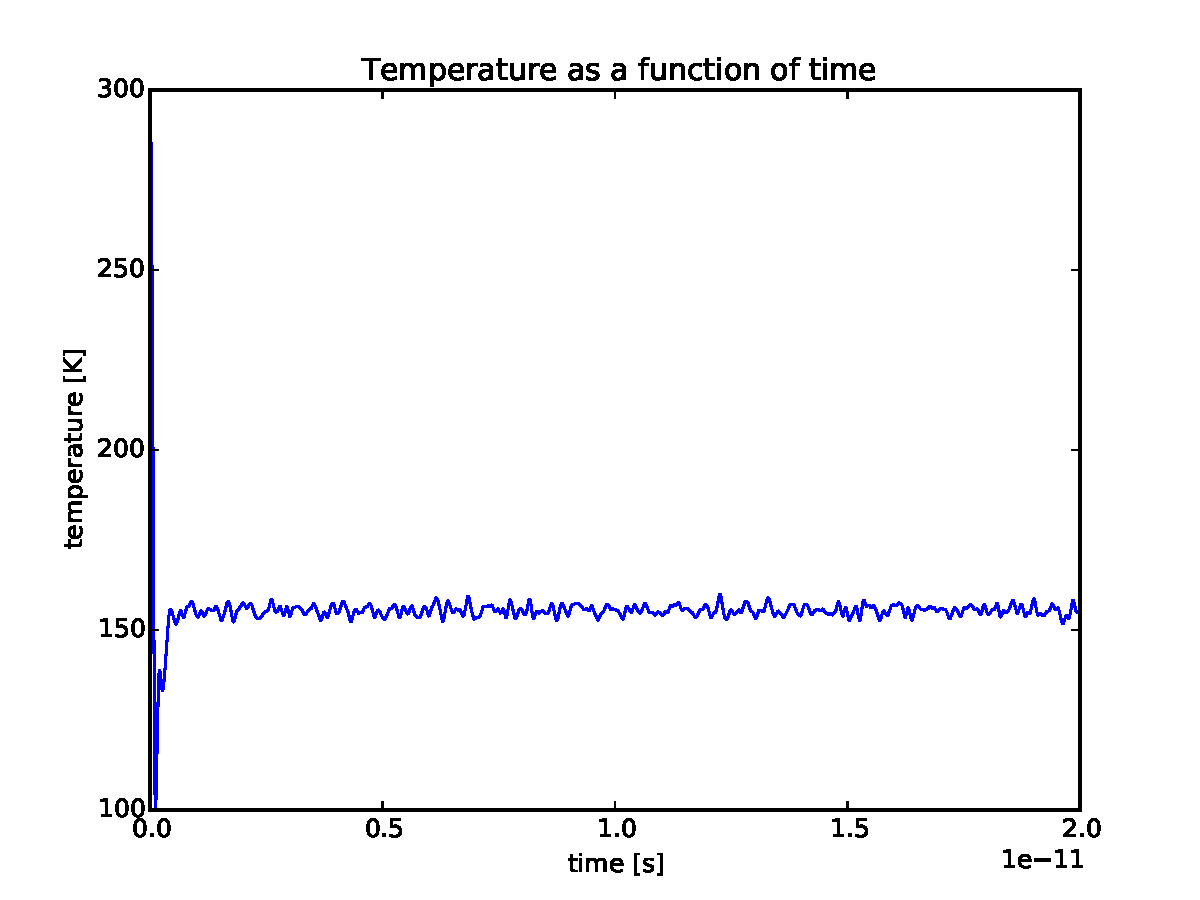
\includegraphics[width=400px]{temperature.pdf}
                \caption{Her har me eit plott som viser korleis temperaturen endrer seg over tid i systemet vårt. Me kan sjå at systemet droppar frå starttemperaturen til
                         ein tredjedel før systemet byrjar å stige mot ein stabil temperatur. Denne er omtrent halvparten av starttemperaturen.}
            \end{figure}
            Atoma er gjevne hastigheitar frå Maxwell-Boltzmann distribusjon i byrjinga. Då $T \propto E_k \propto v^2$, kor $v$ vil vere gjeven frå ein tilfeldig distribusjon
            vil systemet motvirke denne effekten ved å senke temperaturen slik at det vert stabilt. Etterkvart vil systemet nå ein relativt stabil verdi for temperatur. 
            Me veit i tillegg at $T \propto \frac{1}{N}$. Jo fleire atom me har jo mindre fluktuasjonar (mindre amplitude) vil me få for temperaturen.
            Me vil difor, ved bruk av termostat, la systemet få hjelp til å nå den ynskja temperaturen. Når me då slår av termostaten vil me la systemet bruke litt på å 
            stabilisere seg.
            \begin{figure}[H]
                \centering
                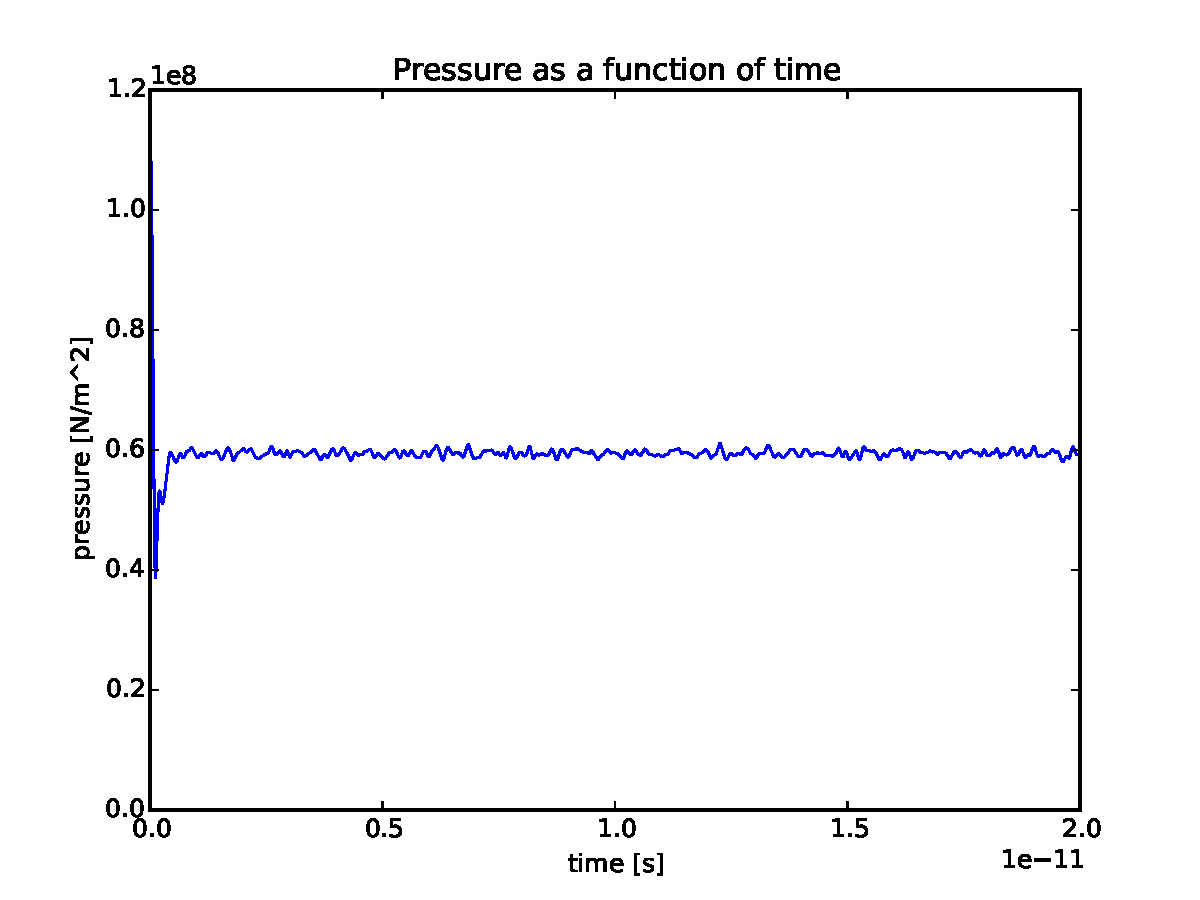
\includegraphics[width=400px]{pressure.pdf}
                \caption{Ikkje overraskande nok vil trykket fylgje ei liknande rørsle som temperaturen då $P \propto T$}
            \end{figure}
            \begin{figure}[H]
                \centering
                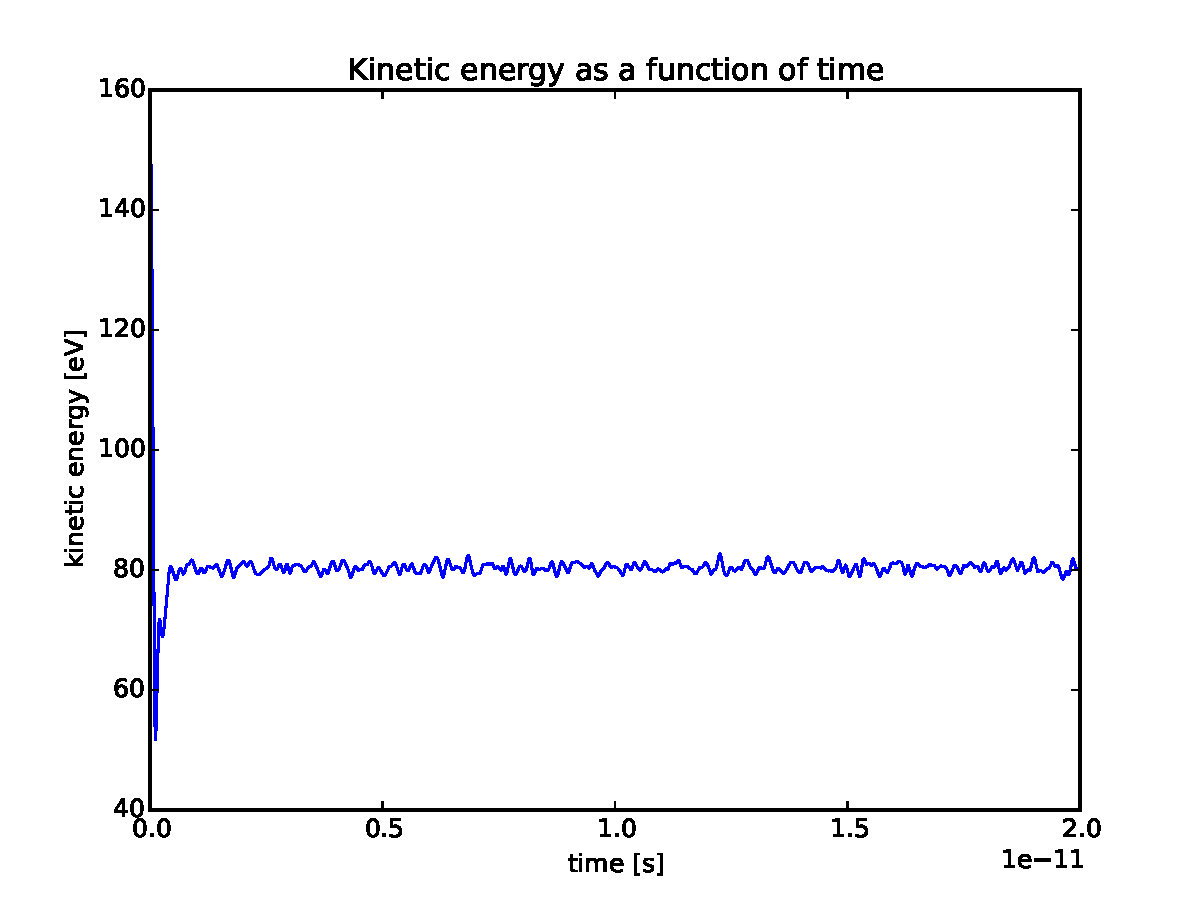
\includegraphics[width=400px]{kineticEnergy.pdf}
                \caption{Då $T \propto E_k$ vil dette og gjere at me kjenner igjen fluktuasjonane frå temperaturplottet.}
            \end{figure}
            \begin{figure}[H]
                \centering
                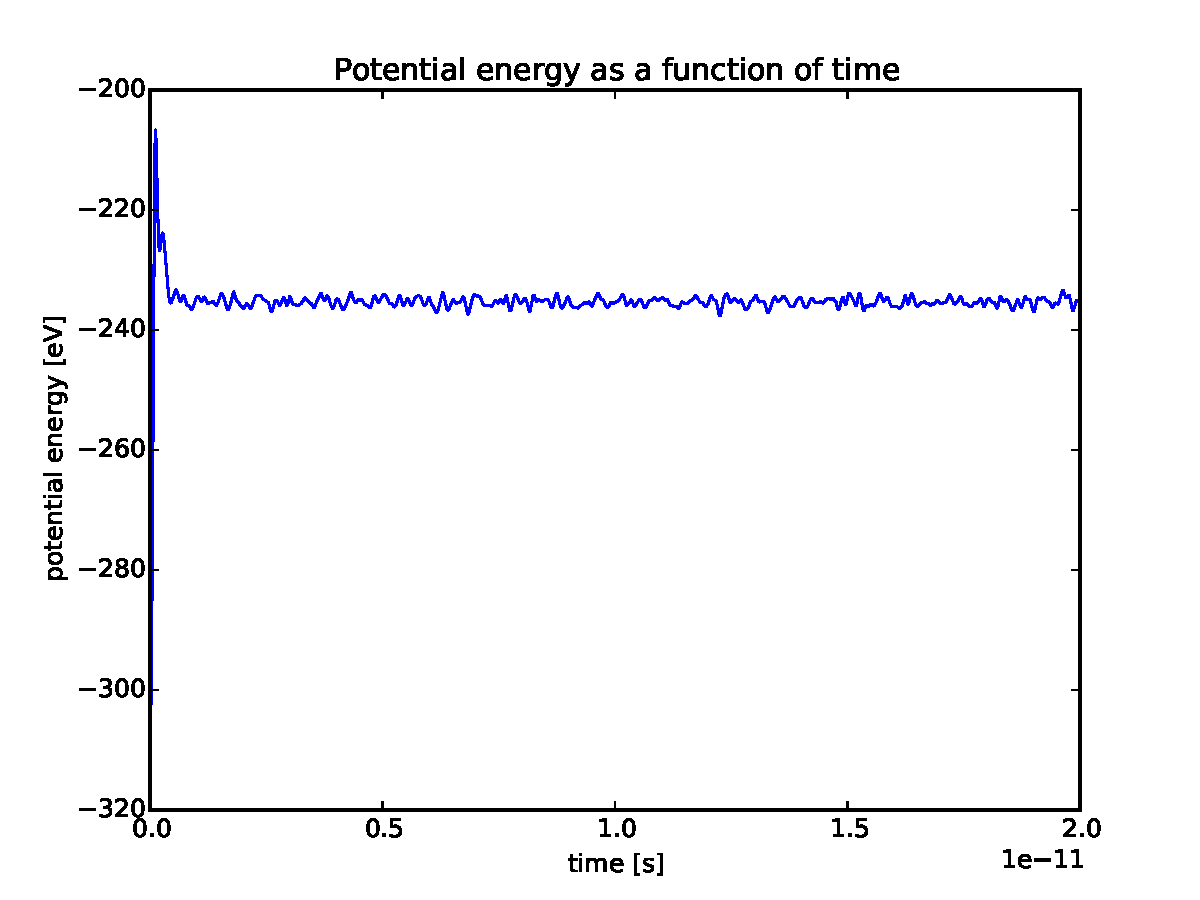
\includegraphics[width=400px]{potentialEnergy.pdf}
                \caption{Siden total energien skal vere bevart må den potensielle energien fluktuere mot den kinetiske energien.}
            \end{figure}
            \begin{figure}[H]
                \centering
                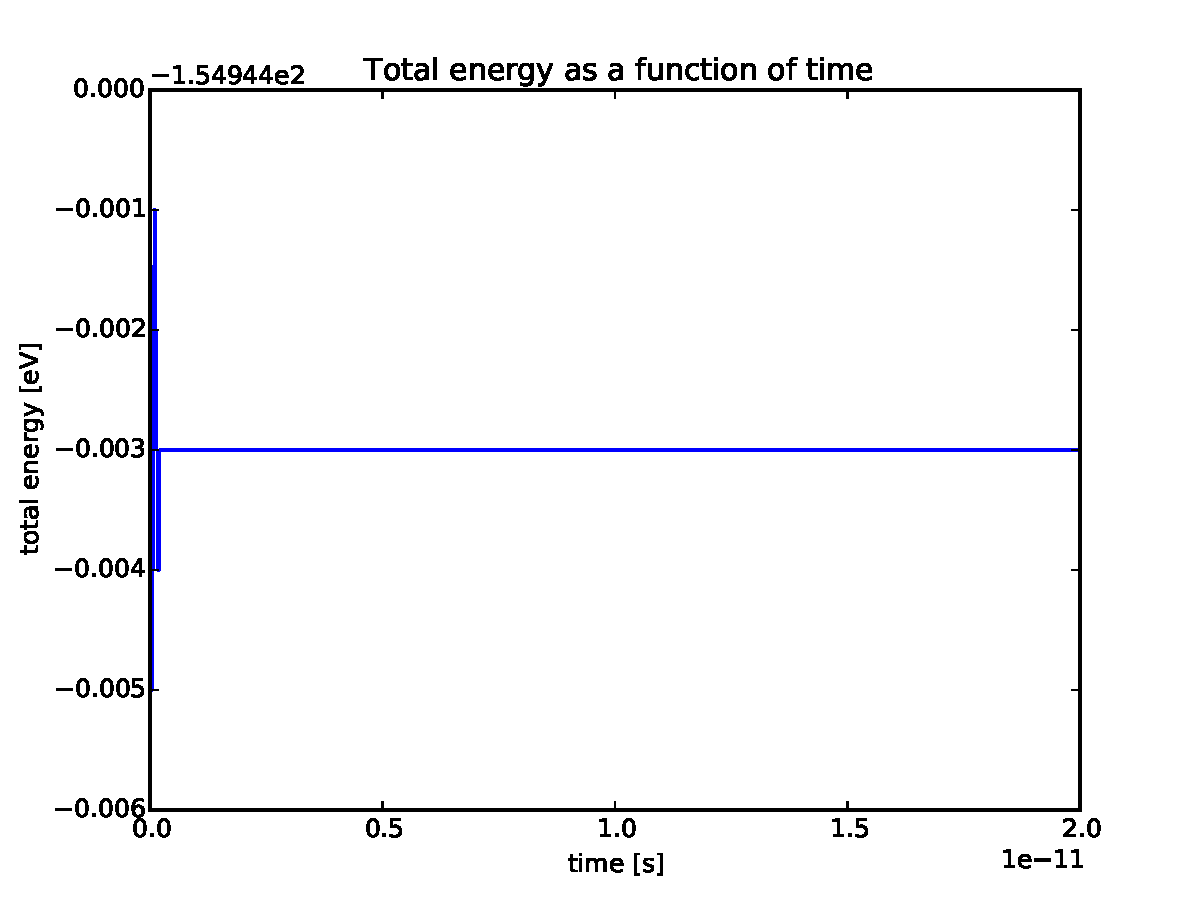
\includegraphics[width=400px]{totalEnergy.pdf}
                \caption{Her kan me sjå at for nokre få startverdiar vil total energien fluktuere i ein magnitude på $1.0\times10^{-3}$. Etterkvart får me ein veldig stabil
                         verdi, slik me ynskjer.}
            \end{figure}

        \subsubsection*{Variasjon i trykk mot tettleiken}
            \addcontentsline{toc}{subsubsection}{Variasjon i trykk mot tettleiken}
    % Hugs å sjå på bevaring av energi for forskjellige val av dt.
    % Legg ved smeltetemperatur og stabilitetstemperatur.
    % Sjå på kvifor temperaturen synker og korleis fluktuasjonar avhenger av antal atom.
    % Sjekk korleis trykket varierer og plott det mot tettleiken.

\end{document}
